% Created 2020-05-20 Wed 18:19
% Intended LaTeX compiler: pdflatex
\documentclass[11pt]{article}
\usepackage[utf8]{inputenc}
\usepackage[T1]{fontenc}
\usepackage{graphicx}
\usepackage{grffile}
\usepackage{longtable}
\usepackage{wrapfig}
\usepackage{rotating}
\usepackage[normalem]{ulem}
\usepackage{amsmath}
\usepackage{textcomp}
\usepackage{amssymb}
\usepackage{capt-of}
\usepackage{hyperref}
\usepackage{minted}
\usepackage[a4paper,margin=20mm]{geometry}
\usepackage{amsmath}
\usepackage{amsfonts}
\usepackage{stmaryrd}
\usepackage{bm}
\usepackage{minted}
\usemintedstyle{emacs}
\usepackage[T1]{fontenc}
\usepackage[scaled]{beraserif}
\usepackage[scaled]{berasans}
\usepackage[scaled]{beramono}
\newcommand{\tr}{\textsf{T}}
\newcommand{\grad}{\bm{\nabla}}
\newcommand{\av}[2][]{\mathbb{E}_{#1\!}\left[ #2 \right]}
\newcommand{\Prob}[2][]{\mathbb{P}_{#1\!}\left[ #2 \right]}
\newcommand{\logg}[1]{\log\!\left( #1 \right)}
\newcommand{\pred}[1]{\left\llbracket { \small #1} \right\rrbracket}
\newcommand{\e}[1]{{\rm e}^{#1}}
\newcommand{\dd}{\mathrm{d}}
\newcommand{\ii}{\mathrm{i}}
\DeclareMathAlphabet{\mat}{OT1}{cmss}{bx}{n}
\newcommand{\normal}[2]{\mathcal{N}\!\left(#1 \big| #2 \right)}
\newcounter{eqCounter}
\setcounter{eqCounter}{0}
\newcommand{\explanation}{\setcounter{eqCounter}{0}\renewcommand{\labelenumi}{(\arabic{enumi})}}
\newcommand{\eq}[1][=]{\stepcounter{eqCounter}\stackrel{\text{\tiny(\arabic{eqCounter})}}{#1}}
\newcommand{\argmax}{\mathop{\mathrm{argmax}}}
\newcommand{\Dist}[2][Binom]{\mathrm{#1}\left( \strut {#2} \right)}
\newcommand{\goesto}[1]{\stackrel{#1}{\longrightarrow}}
\author{Adam Prügel-Bennett}
\date{\today}
\title{Computational Biology Subsidary Notes\\\medskip
\large Lecture 18: Simulating Chemical Equations}
\hypersetup{
 pdfauthor={Adam Prügel-Bennett},
 pdftitle={Computational Biology Subsidary Notes},
 pdfkeywords={},
 pdfsubject={},
 pdfcreator={Emacs 26.3 (Org mode 9.1.9)}, 
 pdflang={English}}
\begin{document}

\maketitle

\section{Keywords}
\label{sec:orgbc4fc3e}
\begin{itemize}
\item Gene regulation, chemical equations, motifs
\end{itemize}

\section{Main Points}
\label{sec:org638acf6}

\subsection{Stochasticity}
\label{sec:orga0d267a}
\begin{itemize}
\item Chemical equations happen by chance interactions of molecules
\begin{itemize}
\item The molecules are moving around due to Brownian motion and when
the right molecules collide with the right energy a reaction happens
\end{itemize}
\item If there are enough molecules then the actual number of molecules
will be close to their mean number and the behaviour is well
described by ordinary differential equations
\item In some biological situations there may be so few molecules of a
specific type that the stochastic nature of the dynamics qualitatively
changes what happens
\item There is considerable research interest as to whether cells can
use this stochasticity for their own purposes
\begin{itemize}
\item For example, in a population of cells you might want some
proportion of cells to respond to a stimulus or to
differentiate
\item This can be achieved if the state of the cell is controlled by
a stochastic process caused by the existence of a very small
number of molecules
\end{itemize}
\item In modelling stochastic behaviour biologists often distinguish
between two different types of randomness
\begin{enumerate}
\item \textbf{Extrinsic Noise}
\begin{itemize}
\item This is noise that is external to the chemical equations
being modelled
\item This might arise due to changes in the number of RNA-polymerase
or ribosomes, or the size of cells
\end{itemize}
\item \textbf{Intrinsic Noise}
\begin{itemize}
\item This is randomness that arises because of stochasticity in
the chemical processes being modelled
\end{itemize}
\end{enumerate}
\end{itemize}

\subsubsection{Probability of a Reaction}
\label{sec:org95f772c}
\begin{itemize}
\item When modelling particular reactions we have to calculate the
probability of the reactants to come together
\item Consider the reaction
\[  2\,X + Y \goesto{k} 3\, X \]
\item We assume that this reaction will only take place if two \(X\)
molecules and one \(Y\) molecule co-exist in a small volume
\(\delta V\)
\begin{center}
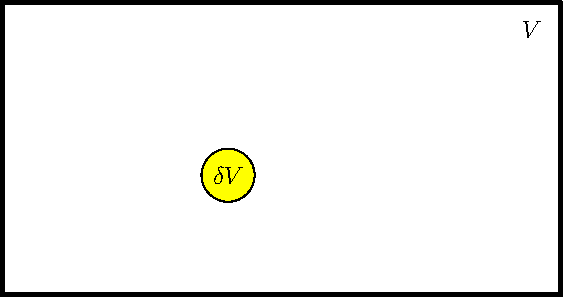
\includegraphics[width=0.25\textwidth]{./figures/smallVolume.pdf}
\end{center}
\item The probability that a particular molecule \(Y_i\) exists in a
small volume, \(\delta V\), is given by \(\Prob{Y_i\in\delta V} = \delta
      V/V\), where \(V\) is the volume of the cell
\item If there are \(n_Y\) molecules of type \(Y\) in the cell, then the
probability of there being at least one molecule in volume
\(\delta V\) is \(n_Y\,\delta V/V = [Y]\,\delta V\) (where \([Y] =
      n_Y/V\) is the concentration of \(Y\))
\item The probability that any two particles \(X_1\) and \(X_2\) say are
both in volume \(V\) at any one time is \((\delta V/V)^2\)
\item If there are \(n_X\) particles of type \(X\) then the probability
that at least two of them are in volume \(\delta V\) is
\[ \frac{m\,(m-1)}{2} \left( \frac{\delta V}{V} \right)^2
      \approx \frac{(\delta V)^2}{2} [X]^2 \]
\item The probability of at least one particle of type \(Y\) and two
particles of type \(X\) are in volume \(\delta V\) is
\[ \frac{(\delta V)^3}{2} \,[Y]\,[X]^2  \]
\item There are \(V/(\delta V)\) volumes of size \(\delta V\) in our cell
of volume \(V\)
\item Thus the probability that in one of these volumes there are two
molecules of type \(X\) and one of type \(Y\) is
\[ \frac{V\,(\delta V)^2}{2} \,[Y]\,[X]^2  \]
\item The reaction rate \(k\) of this reaction is defined so that the
probability of there being a reaction in time \(\delta t\) per
unit volume is
\[ k\,[Y]\,[X]^2 \, \delta t\]
\begin{itemize}
\item Note that \(k\) is defined to absorb the combinatorial function \(\tfrac{1}{2}\)
\item The rate will depend on how close together the molecules have
to be for a reaction to occur (i.e. on \(\delta V\))
\item There will be other factors such as the orientation of the
molecules and the relative velocity of the molecules
\item From a chemical point of view, \(k\), would measure the reaction
rate per litre if all the reactants were 1 molar solutions (1
moles of \(X\) and \(Y\) per litre (dm\(^{3}\)))
\end{itemize}
\item To model small numbers of molecules we have to work with the
number of molecules \(n_X\), \(n_Y\), etc.
\item We note that \([X] = n_X/(N_A\,V)\) where \(N_A\) is Avogadro's
number and \(V\) is the volume of the cell (we frequently write
\(\Omega = N_A\,V\))
\item If we have a reaction \(2\,X + Y \goesto{k} 3\, X\)
then the change in concentration per unit time is \(k\, [Y]\,[X]^2\)
\item Multiply this rate by \(\Omega = N_A\,V\) we get the expected number of
reactions in a cell of volume \(V\) per unit time
\item Thus the probability of this reaction occurring in time \(\delta t\) is
\[ \frac{k}{\Omega^2} \, n_Y \, n_X^2 \, \delta t \]
\item If we wanted to be more precise (which might be important if we
have a very small number of \(X\) molecules) then this probability
is
 \[ \frac{k}{\Omega^2} \, n_Y \, n_X\,(n_X-1)\, \delta t \]
\end{itemize}

\subsection{Gillespie Algorithm}
\label{sec:orgb2fb7bc}
\begin{itemize}
\item We can simulate dynamics of a molecular system when we
have a small number of molecules
\begin{itemize}
\item This is just one instance of what might happen (next time we do
the simulation we would get a different dynamics)
\end{itemize}
\item Let's consider the system
\begin{align*}
  \varnothing &\goesto{k_1} A  &
  \varnothing &\goesto{k_2} B & 
   A + B &\goesto{k_3} C &
   C &\goesto{k_4} A + B
\end{align*}
\item We let \(n_A(t)\), \(n_B(t)\) and \(n_C(t)\) be the number of molecules
of type \(A\), \(B\) and \(C\) at time \(t\)
\item We are going to assume that the reactions are so fast that they happen instantly
\item In the theory of stochastic processes these are known as \textbf{point processes}
\item Now the probability of a reaction occurring it time \(\delta t\) is
\begin{align*}
\Prob{\varnothing \goesto{k_1} A} &= k_1\,\delta t  = a_1(\bm{X}(t))\, \delta t\\
\Prob{\varnothing \goesto{k_2} B} &= k_2\,\delta t = a_2(\bm{X}(t))\, \delta t \\
\Prob{A + B \goesto{k_3} C} &= \frac{k_3}{\Omega}\,n_{A}\,n_{B}\,\delta t = a_3(\bm{X}(t))\, \delta t \\
\Prob{C \goesto{k_4} A + B} &= k_4\,n_C\,\delta t  = a_4(\bm{X}(t))\, \delta t
\end{align*}
\item \(a_i(\bm{X}(t))\) are known as the \textbf{propensity} of reaction \(i\)
\item Many of the propensity will change after each reaction
\item \textbf{Gillespie's algorithm} simulates a chemical process one reaction
at a time
\begin{itemize}
\item From the propensities it draws a random time interval, \(T\), to
the next chemical reaction
\item We then randomly decides which chemical reaction takes place
\item We then updates the propensities
\end{itemize}
\item What is surprising is just how easy it is to simulate chemical
equations using Gillespie's algorithm
\end{itemize}

\subsubsection{Poisson Process}
\label{sec:org764d3d7}
\begin{itemize}
\item In modelling chemical equations each reaction happens
independently at each time interval
\item As a consequence our point process becomes a \textbf{Poisson process}
(the simplest type of point process)
\item We suppose we have a point process with a probability of occurring
in time \(\delta t\) of \(a\, \delta t\)
\item The probability of the first occurrence happening in time interval
\(n\,\delta t \leq t \leq (n+1)\,\delta t\) is
\begin{align*}
\Prob{n\,\delta t \leq t \leq (n+1)\,\delta t}
&\eq (1-a \,\delta t)^n \,a \, \delta\,t
\eq a \, \e{n\log(1-a \,\delta t)} \, \delta t\\
&\eq[\approx] a \, \e{-a\,n \,\delta t} \, \delta t
\eq[\approx] a \, \e{-a\,t} \, \delta t
\end{align*}
\explanation
\begin{enumerate}
\item This is the probability that it doesn't happen, \(1-a\,\delta
	 t\), in the previous \(n\) time intervals times the probability
that it does happen, \(a\,\delta t\)
\item Using \(x^n = \e{n\,\log(x)}\)
\item Since \(\log(1+\Delta) \approx \Delta +O(\Delta^2)\)
\item Using \(n\,\delta t \approx t\)
\end{enumerate}
\item Taking the limit \(\delta t\rightarrow 0\) then the probability
density for the next time an event occurs is
\begin{align*}
f_T(t) = \lim_{\delta t\rightarrow 0} \frac{\Prob{n\,\delta
t \leq t \leq (n+1)\,\delta t}}{\delta t}= a\,\e{-a\,t}
\end{align*}
\item In modelling a series of \(K\) chemical equations where the
probability of reaction \(i\) occurring in time \(\delta t\) is
\(a_i\,\delta t\) then the probability of any one reaction
occurring in this time interval is \(a_0 \,\delta t\) where
\(a_0=\sum_{i=1}^K a_i\)
\item If \(T\) is a random variable equal to the time until the next
reaction then it will be distributed according to the probability
density
\[ f_T(t) = a_0\,\e{-a_0\,t} \]
\item The probability that when a reaction happens
that it is reaction \(i\) is
\begin{align*}
\Prob{\text{reaction $i$ happens}} =
\frac{a_i}{a_1+\cdots+a_K} = \frac{a_i}{a_0}
\end{align*}
\item We now need to be able draw random deviates from an exponential distribution
\item We first consider the case when \(a_{0}=1\) so that \(f_T(t) =
      \mathrm{Exp}(t) = \e{-t}\)
\item The trick to drawing a random deviate from this distribution is
to invert the cumulative probability distribution
\[ F_T(t) = \int_0^t \, \mathrm{Exp}(\tau) \, \dd \tau =
      1-\e{-t} \]
\item So that \(F^{-1}_T(x) = -\log(1-x)\)
\item Now if we choose a uniform random deviate \(U\sim
      \mathrm{Uni}(0,1)\) between 0 and 1 then
\[ T = F^{-1}_T(U) \]
will be exponentially distributed
\begin{itemize}
\item We can prove this, but this goes beyond what you need to know
for the course
\item Let's consider the probability that \(T\) is between \(t\) and
\(t + \delta t\)
\[ \Prob{t\leq T \leq t+\delta t} = \int_0^1 \pred{t\leq
        F^{-1}_T(u)\leq t +\delta t}\, \dd u \]
\item where \(\pred{\text{predicate}} = 1\) if \emph{predicate} is true and
0 otherwise
\item But we can rewrite this as
\[ \Prob{t\leq T \leq t+\delta t} = \int_{F_T(t)}^{F_T(t+\delta
        t)} \,\dd u = F_T(t+\delta t) - F_T(t) \]
\begin{itemize}
\item You can convince yourself that for \(u\in[F_T(t),F_T(t+\delta
          t)]}\) we have \(t\leq F_T^{-1}(u)\leq t + \tau\)
\end{itemize}
\item Using the Taylor expansion \(F_T(t+\delta t)  = F_T(t) + \delta t
        \, F_{T}'(t) + O(\delta t^2)\)
\item But \(F_T'(t) = f_T(t)\) that is, the derivative of a cumulative
distribution function (CDF) is equal to the probability
density function (PDF)
\item Thus \(\Prob{t\leq T \leq t+\delta t}/\delta t = f_{T}(t) +
        O(\delta t)\)
\item Taking the limit when \(\delta t\rightarrow0\) we see that \(T\)
has a probability density \(f_T(t)\)
\end{itemize}
\item To draw a random deviate \(T \sim \mathrm{Exp}(t|a) =
       a\,\exp(-a\,t)\) we just make the change of variable from \(T\) to \(T/a\)
\item That is, we choose \(T = -\log(1-U)/a\)
\item For the Gillespie algorithm with molecule species \(\bm{X}(t) =
      (X_1(t),\,X_2(t),\,\ldots,\,X_N(t))\) where we have \(K\) reactions
with propensities \(a_i(\bm{X}(t))\) we do the following
\begin{enumerate}
\item Compute the total propensity \(a_0(\bm{X}(t)) = \sum_{j=1}^K
         a_i(\bm{X}(t))\)
\item Draw a random time \(T\sim \mathrm{Exp(t|a_0)}\) using
\[ T &= - \frac{1}{a_0(\bm{X}(t))} \log(1-U) & U&\sim\mathrm{Uni}(0,1) \]
\item Select the reaction that happened with probabilities
\[ \Prob{j} = \frac{a_j(\bm{X}(t))}{a_0(\bm{X}(t))} \]
\item Update time \(t\rightarrow t + T\)
\item Update the molecular numbers according to the reaction that
has taken place
\end{enumerate}
\item For the example we discussed previously
 \begin{align*}
  \varnothing &\goesto{0.05} A  &
  \varnothing &\goesto{0.03} B & 
  A + B &\goesto{0.005/\Omega} C &
  C &\goesto{0.01} A + B
\end{align*}
\begin{center}
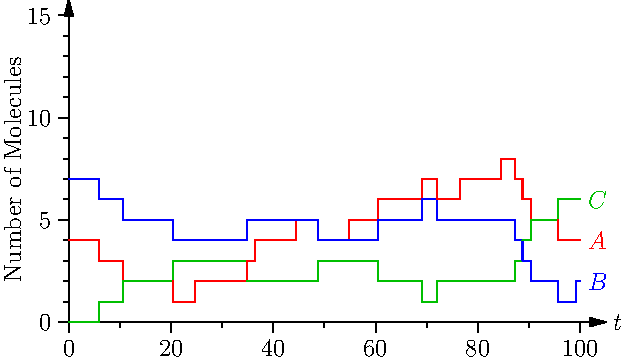
\includegraphics[width=0.5\textwidth]{./figures/reactions-20.pdf}
\end{center}
\item As a second example consider the two species system we studied
in the last lecture
\begin{align*}
\varnothing &\goesto{f(X_2)} X_1 &
X_1 &\goesto{k_3} \varnothing & X_1 &\goesto{k_5} X_2 \\
\varnothing &\goesto{k_2} X_2 & X_2 &\goesto{k_4} \varnothing &&
\end{align*}
\begin{itemize}
\item Here \(X_2\) represses the expression of \(X_1\) according to the
Hill equation for a repressor
\begin{align*}
f(X_2) &= \frac{k_1}{1+(X_2/K)^n}\pause
\end{align*}
\item Leading to the coupled ODEs
\begin{align*}
 \frac{\dd [X_1(t)]}{\dd t} &= \frac{k_1}{1+([X_2(t)]/K)^n} - k_3 \,
                           [X_1(t)]- k_5\,[X_1(t)] \\
  \frac{\dd [X_2(t)]}{\dd t} &= k_2 + k_5\,[X_1(t)] - k_4\,[X_2(t)]
\end{align*}
\item We can solve the ODEs giving a dynamics for \(K=1\), \(k_1=20\),
\(k_2=k_3=k_4=5\), \(k_5=2\), \(n=4\)
\begin{center}
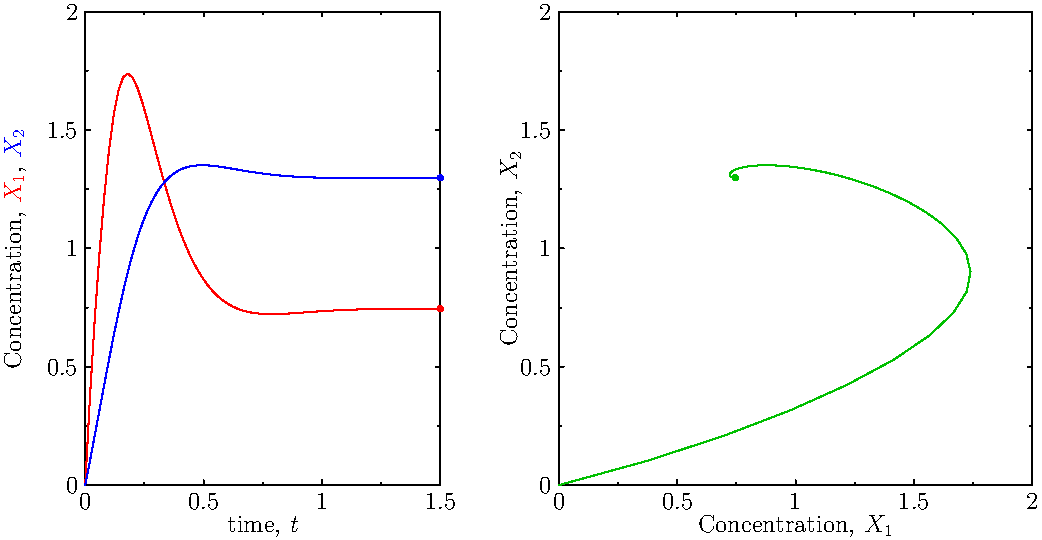
\includegraphics[width=0.5\textwidth]{./figures/coupledODE-41.pdf}
\end{center}
\item If we change the units of concentration so that \([X_i(t)]
        \rightarrow r\,[X_i(t)]\) this would lead to a  change in the differential equations
\item But if we rescale the reaction rates appropriately \(K\rightarrow r\,K\),
\(t\rightarrow r\,t\), \(k_i\rightarrow k_i/r\) for
\(i\in\{3,4,5\}\) this leaves the ODEs invariant
\item This allows us to simulate the system with the same mean
dynamics but with different number of molecules in the finite
molecule simulation (this is entirely artificial in any real
biological system the reaction rates and cell volume are given)
\item Using \(r=1000\) we can simulate the dynamics as shown in figure \ref{fig:large}
\begin{figure}[htbp]
\centering
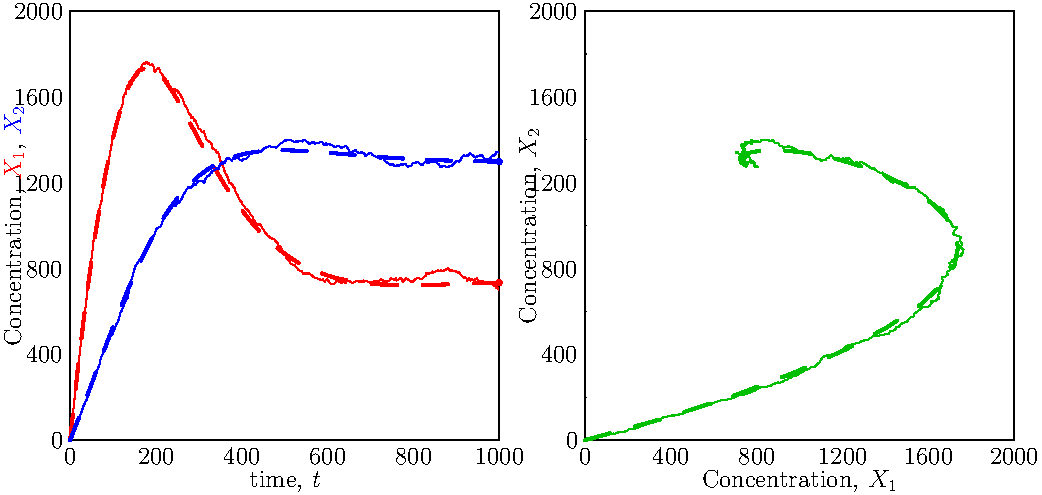
\includegraphics[width=0.5\textwidth]{./figures/GillespieLarge-39.pdf}
\caption{Gillespie dynamics using \(r=1000\) \label{fig:large}}
\end{figure}
\item The dashed curves in figure \ref{fig:large} shows the ODE solution
\item The continuous curve shows the Gillespie dynamics
\item Using this value of \(r\) then \(K=1000\), \(k_1=0.02\),
\(k_2=k_3=k_4=0.005\), \(k_5=0.002\) and \(n=4\) and the time is in
measured in units of 1000 second
\item Using \(r=100\) we can simulate the dynamics as shown in figure \ref{fig:medium}
\begin{figure}[htbp]
\centering
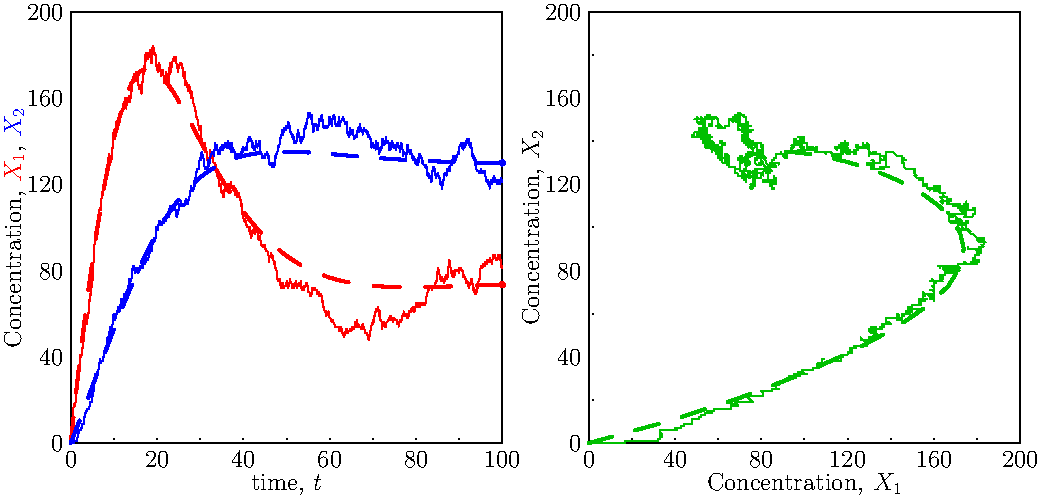
\includegraphics[width=0.5\textwidth]{./figures/GillespieMedium-39.pdf}
\caption{Gillespie dynamics using \(r=100\) \label{fig:medium}}
\end{figure}
\item Using \(r=10\) we can simulate the dynamics as shown in figure \ref{fig:small}
\begin{figure}[htbp]
\centering
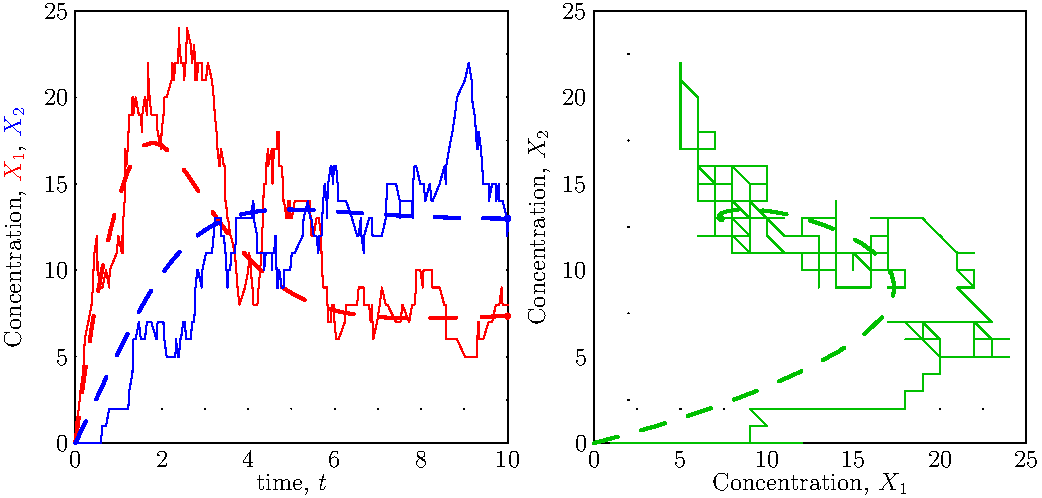
\includegraphics[width=0.5\textwidth]{./figures/GillespieSmall-39.pdf}
\caption{Gillespie dynamics using \(r=10\) \label{fig:small}}
\end{figure}
\item This shows how when we have a smaller number of molecules the
ODEs can provide a poor description of what goes on
\item If we have a stable fixed-points with a small basin of attraction often
these fluctuations mean that the system always escapes from
this fixed point
\item Occasionally these fluctuations can cause a random
flip-flopping between different fixed-points
\end{itemize}
\item Gillespie is very efficient and can simulate systems with a
millions of molecules
\item However, we can easily have systems where we have too many molecules
for Gillespie to be feasible (Avogadro's number is very large)
\item Usually this doesn't matter because this is the regime where the
ODEs work
\item There can be times where some molecules are very common and
others very rare in which case we often need to use tricks so we
can simulate the rare molecules using Gillespie, but use some
other approximation to simulate the other species of molecules
\end{itemize}
\end{document}
